\documentclass{beamer}

\usepackage{subfigure}
\usepackage[english]{babel}
\usepackage[latin1]{inputenc}
\usepackage{times}
\usepackage[T1]{fontenc} 
\usepackage{color}

\usepackage{algorithm}
\usepackage{algorithmicx}
\usepackage[noend]{algpseudocode}

\usetheme[secheader]{Boadilla}
\usefonttheme[onlylarge]{structurebold}
\setbeamerfont*{frametitle}{size=\normalsize,series=\bfseries}
\setbeamertemplate{navigation symbols}{}
\setbeamertemplate{mini frames}[box]
\setbeamertemplate{sections/subsections in toc}[square]
\setbeamertemplate{blocks}[rounded][shadow=true]
\setbeamertemplate{bibliography item}[text]

\setbeamercolor{lightorange}{fg=black,bg=orange!40}
\setbeamercolor{lightblue}{fg=black,bg=blue!30}

\newenvironment{colorblock}[2]
{\setbeamercolor{item}{fg=#1,bg=#1}\begin{beamerboxesrounded}[upper=#1,lower=#2,shadow=true]}
  {\end{beamerboxesrounded}}



% Setup TikZ

\usepackage{tikz}
\usetikzlibrary{arrows}
\tikzstyle{block}=[draw opacity=0.7,line width=1.4cm]


%%%%%%%%%%%%%%%%%%%%%%%%%%%%%%%%%%%%%
%%%%%%%%%%%%%%%%%%%%%%%%%%%%%%%%%%%%%
%%%%%%%%%%%%%%%%%%%%%%%%%%%%%%%%%%%%%

\newtheorem{observation}[theorem]{Observation} 

%%%%%%%%%%%%%%%%%%%%%%%%%%%%%%%%%%%%%
%%%%%%%%%%%%%%%%%%%%%%%%%%%%%%%%%%%%%
%%%%%%%%%%%%%%%%%%%%%%%%%%%%%%%%%%%%%

\title{Relational Algebra and MapReduce}
\subtitle{Towards High-level Programming Languages}
\author{Pietro Michiardi}
\institute{Eurecom}
\date


\begin{document}

\begin{frame}
  \titlepage
\end{frame}

%%%%%%%%%%%%%%%%%%%%%%%%%%%%%%%%%%%%%%%%%%%%%%%%%%%%%%%%%%
\section{Sources and Acks}

\begin{frame}
  \begin{itemize}
    \item Jimmy Lin and Chris Dyer, ``Data-Intensive Text Processing with MapReduce,'' Morgan \& Claypool Publishers, 2010. \url{http://lintool.github.io/MapReduceAlgorithms/}

    \item[]

    \item Tom White, ``Hadoop, The Definitive Guide,'' O'Reilly / Yahoo Press, 2012

    \item[]

    \item Anand Rajaraman, Jeffrey D. Ullman, Jure Leskovec, ``Mining of Massive Datasets'', Cambridge University Press, 2013
  \end{itemize}
\end{frame}

%%%%%%%%%%%%%%%%%%%%%%%%%%%%%%%%%%%%%%%%%%%%%%%%%%%%%%%%%%


%%%%%%%%%%%%%%%%%%%%%%%%%%%%%%%%%%%%%%%%%%%%%%%%%%%%%%%%%%
\section{Relational Algebra}

\begin{frame}
 \begin{colorblock}{blue}{lightblue}{ }
  \begin{center}
    \Huge \textbf{\texttt{Relational Algebra and MapReduce}}
  \end{center}
  \end{colorblock}
\end{frame}

%%%%%%%%%%%%%%%%%%%%%%%%%%%%%%%%%%%%%%%%%%%%%%%%%%%%%%%%%%
%%%%%%%%%%%%%%%%%%%%%%%%%%%%%%%%%%%%%%%%%%%%%%%%%%%%%%%%%%
\subsection{Introduction}
%%%%%%%%%%%%%%%%%%%%%%%%%%%%%%%%%%%%%%%%%%%%%%%%%%%%%%%%%%
%%%%%%%%%%%%%%%%%%%%%%%%%%%%%%%%%%%%%%%%%%%%%%%%%%%%%%%%%%


%%%%%%%%%%%%%%%%%%%%%%%%%%%%%%%%%%%%%%%%%%%%%%%%%%%%%%%%%%
\frame {\frametitle{Introduction}
%%%%%%%%%%%%%%%%%%%%%%%%%%%%%%%%%%%%%%%%%%%%%%%%%%%%%%%%%%
  \begin{itemize}
  \item \textbf{Disclaimer}
    \begin{itemize}
    \item This is not a full course on Relational Algebra
    \item Neither this is a course on SQL
    \end{itemize}

    \vspace{20pt}

  \item \textbf{Introduction to Relational Algebra, RDBMS and SQL}
    \begin{itemize}
    \item Follow the video lectures of the Stanford class on RDBMS
    \item[] \url{https://www.coursera.org/course/db}
    \item[$\to$] Note that you have to sign up for an account
    \end{itemize}

    \vspace{20pt}

  \item \textbf{Overview of this part}
    \begin{itemize}
    \item Brief introduction to simplified relational algebra
    \item Useful to understand Pig, Hive and HBase
    \end{itemize}

  \end{itemize}
}

%%%%%%%%%%%%%%%%%%%%%%%%%%%%%%%%%%%%%%%%%%%%%%%%%%%%%%%%%%
\frame {\frametitle{Relational Algebra Operators}
%%%%%%%%%%%%%%%%%%%%%%%%%%%%%%%%%%%%%%%%%%%%%%%%%%%%%%%%%%
  \begin{itemize}
  \item \textbf{There are a number of operations on data that fit well
      the relational algebra model}
    \begin{itemize}
    \item In traditional RDBMS, queries involve retrieval of
      {\color{red}small amounts of data}
    \item In this course, and in particular in this class, we should
      keep in mind the particular workload underlying MapReduce
    \item[$\to$] Full scans of large amounts of data
    \item[$\to$] Queries are not selective\footnote{This is true in general. However, most ETL jobs involve selection and projection to do data preparation.}, they process all data
    \end{itemize}

    \vspace{20pt}

  \item \textbf{A review of some terminology}
    \begin{itemize}
    \item A {\color{red}\textit{relation}} is a table
    \item {\color{red}\textit{Attributes}} are the column headers of
      the table
    \item The set of attributes of a relation is called a
      {\color{red}\textit{schema}}
    \item[] Example: $R(A_1,A_2,...,A_n)$ indicates a relation called
      $R$ whose attributes are $A_1,A_2,...,A_n$
    \end{itemize}
  \end{itemize}
}



%%%%%%%%%%%%%%%%%%%%%%%%%%%%%%%%%%%%%%%%%%%%%%%%%%%%%%%%%%
%%%%%%%%%%%%%%%%%%%%%%%%%%%%%%%%%%%%%%%%%%%%%%%%%%%%%%%%%%
\subsection{Operators}
%%%%%%%%%%%%%%%%%%%%%%%%%%%%%%%%%%%%%%%%%%%%%%%%%%%%%%%%%%
%%%%%%%%%%%%%%%%%%%%%%%%%%%%%%%%%%%%%%%%%%%%%%%%%%%%%%%%%%

%%%%%%%%%%%%%%%%%%%%%%%%%%%%%%%%%%%%%%%%%%%%%%%%%%%%%%%%%%
\frame {\frametitle{Operators}
%%%%%%%%%%%%%%%%%%%%%%%%%%%%%%%%%%%%%%%%%%%%%%%%%%%%%%%%%%
  \begin{itemize}
  \item \textbf{Let's start with an example}
    \begin{itemize}
    \item Below, we have part of a relation called \textit{Links}
      describing the structure of the Web
    \item There are two \textit{attributes}: \textit{From} and
      \textit{To}
    \item A row, or {\color{red}\textit{tuple}}, of the relation is a
      pair of URLs, indicating the existence of a link between them
    \item[$\to$] The number of tuples in a real dataset is in the
      order of billions ($10^9$)
    \end{itemize}
  \end{itemize}
  
  \begin{center}
    \begin{tabular}[h]{|c|c|}
      \hline
      From & To \\
      \hline
      \hline
      \texttt{url1} & \texttt{url2} \\
      \texttt{url1} & \texttt{url3} \\
      \texttt{url2} & \texttt{url3} \\
      \texttt{url2} & \texttt{url4} \\
      $\cdots$ & $\cdots$\\
      \hline
    \end{tabular}   
  \end{center}
}

%%%%%%%%%%%%%%%%%%%%%%%%%%%%%%%%%%%%%%%%%%%%%%%%%%%%%%%%%%
\frame {\frametitle{Operators}
%%%%%%%%%%%%%%%%%%%%%%%%%%%%%%%%%%%%%%%%%%%%%%%%%%%%%%%%%%
  \begin{itemize}
  \item \textbf{Relations (however big) can be stored in a distributed
      filesystem}
    \begin{itemize}
    \item If they don't fit in a single machine, they're broken into
      pieces (think HDFS)
    \end{itemize}

    \vspace{20pt}

  \item \textbf{Next, we review and describe a set of relational
      algebra operators}
    \begin{itemize}
    \item Intuitive explanation of what they do
    \item ``Pseudo-code'' of their implementation in/by MapReduce
    \end{itemize}
  \end{itemize}
}

%%%%%%%%%%%%%%%%%%%%%%%%%%%%%%%%%%%%%%%%%%%%%%%%%%%%%%%%%%
\frame {\frametitle{Operators}
%%%%%%%%%%%%%%%%%%%%%%%%%%%%%%%%%%%%%%%%%%%%%%%%%%%%%%%%%%
  \begin{itemize}
  \item \textbf{Selection: $\sigma_C(R)$}
    \begin{itemize}
    \item Apply condition $C$ to each tuple of relation $R$
    \item Produce in output a relation containing only tuples that
      satisfy $C$
    \end{itemize}

    \vspace{10pt}

  \item \textbf{Projection: $\pi_S(R)$}
    \begin{itemize}
    \item Given a \textit{subset} $S$ of relation $R$ attributes
    \item Produce in output a relation containing only tuples for
      the attributes in $S$
    \end{itemize}

    \vspace{10pt}

  \item \textbf{Union, Intersection and Difference}
    \begin{itemize}
    \item Well known operators on sets
    \item Apply to the set of tuples in two relations that have the
      {\color{red}same schema}
    \item Variations on the theme: work on \textit{bags}
    \end{itemize}

  \end{itemize}
}

%%%%%%%%%%%%%%%%%%%%%%%%%%%%%%%%%%%%%%%%%%%%%%%%%%%%%%%%%%
\frame {\frametitle{Operators}
%%%%%%%%%%%%%%%%%%%%%%%%%%%%%%%%%%%%%%%%%%%%%%%%%%%%%%%%%%
  \begin{itemize}
  \item \textbf{Natural join $R \Join S$}
    \begin{itemize}
    \item Given two relations, \textit{compare each pair of tuples},
      one from each relation
    \item If the tuples agree on all the attributes common to both
      schema $\to$ produce an output tuple that has components on each
      attribute
    \item Otherwise produce nothing
    \item {\color{red}\textit{Join condition}} can be on a subset of attributes
    \end{itemize}

    \vspace{20pt}

  \item \textbf{Let's work with an example}
    \begin{itemize}
    \item Recall the \textit{Links} relation from previous slides
    \item \texttt{Query} (or data processing job): \texttt{find the paths of length two
      in the Web}
    \end{itemize}
  \end{itemize}
}

%%%%%%%%%%%%%%%%%%%%%%%%%%%%%%%%%%%%%%%%%%%%%%%%%%%%%%%%%%
\frame {\frametitle{Join Example}
%%%%%%%%%%%%%%%%%%%%%%%%%%%%%%%%%%%%%%%%%%%%%%%%%%%%%%%%%%
  \begin{itemize}
  \item \textbf{Informally, to satisfy the query we must:}
    \begin{itemize}
    \item find the triples of URLs in the form $(u,v,w)$ such that
      there is a link from $u$ to $v$ and a link from $v$ to $w$
    \end{itemize}

    \vspace{20pt}

  \item \textbf{Using the join operator}
    \begin{itemize}
    \item Imagine we have two relations (with different schema), and
      let's try to apply the natural join operator
    \item There are two copies of \textit{Links}: $L_1(U_1,U_2)$ and
      $L_2(U_2,U_3)$
    \item Let's compute $L_1 \Join L_2$
      \begin{itemize}
      \item For each tuple $t_1$ of $L_1$ and each tuple $t_2$ of
        $L_2$, see if their $U_2$ component are the same
      \item If yes, then produce a tuple in output, with the schema $(U_1,U_2,U_3)$
      \end{itemize}
    \end{itemize}

  \end{itemize}
}

%%%%%%%%%%%%%%%%%%%%%%%%%%%%%%%%%%%%%%%%%%%%%%%%%%%%%%%%%%
\frame {\frametitle{Join Example}
%%%%%%%%%%%%%%%%%%%%%%%%%%%%%%%%%%%%%%%%%%%%%%%%%%%%%%%%%%
  \begin{itemize}
  \item \textbf{What we have seen is called (to be precise) a
      {\color{red}self-join}}
    \begin{itemize}
    \item {\color{red}Question}: How would you implement a self join in your favorite programming language?
    \item {\color{red}Question}: What is the time complexity of your
      algorithm?
    \item {\color{red}Question}: What is the space complexity of your
      algorithm?
    \end{itemize}

    \vspace{20pt}

  \item \textbf{To continue the example}
    \begin{itemize}
    \item Say you are not interested in the entire two-hop path but
      just the start and end nodes
    \item Then you do a projection and the notation would be:
      $\pi_{U_1,U_3}(L_1 \Join L_2)$
    \end{itemize}
  \end{itemize}

}

%%%%%%%%%%%%%%%%%%%%%%%%%%%%%%%%%%%%%%%%%%%%%%%%%%%%%%%%%%
\frame {\frametitle{Operators}
%%%%%%%%%%%%%%%%%%%%%%%%%%%%%%%%%%%%%%%%%%%%%%%%%%%%%%%%%%
  \begin{itemize}
  \item \textbf{Grouping and Aggregation: $\gamma_X(R)$}
    \begin{itemize}
    \item Given a relation $R$, partition its tuples according to
      their values in one set of attributes $G$
      \begin{itemize}
      \item The set $G$ is called the {\color{red}grouping attributes}
      \end{itemize}
    \item Then, for each group, aggregate the values in certain other
      attributes
      \begin{itemize}
      \item Aggregation functions: \texttt{SUM}, \texttt{COUNT}, \texttt{AVG}, \texttt{MIN}, \texttt{MAX}, ...
      \end{itemize}
    \end{itemize}

    \vspace{20pt}

  \item \textbf{In the notation, $X$ is a list of elements that can be:}
    \begin{itemize}
    \item A grouping attribute
    \item An expression $\theta(A)$, where $\theta$ is one of the
      (five) aggregation functions and $A$ is an attribute
      {\color{red}NOT} among the grouping attributes 
    \end{itemize}

  \end{itemize}

}

%%%%%%%%%%%%%%%%%%%%%%%%%%%%%%%%%%%%%%%%%%%%%%%%%%%%%%%%%%
\frame {\frametitle{Operators}
%%%%%%%%%%%%%%%%%%%%%%%%%%%%%%%%%%%%%%%%%%%%%%%%%%%%%%%%%%
  \begin{itemize}
  \item \textbf{Grouping and Aggregation: $\gamma_X(R)$}
    \begin{itemize}
    \item The result of this operation is a relation with one tuple
      for each group
    \item That tuple has a component for each of the grouping
      attributes, with the value common to tuples of that group
    \item That tuple has another component for each aggregation, with
      the aggregate value for that group
    \end{itemize}

    \vspace{20pt}

  \item \textbf{Let's work with an example}
    \begin{itemize}
    \item Imagine that a social-networking site has a relation
    \item[] \texttt{Friends(User, Friend)}
    \item The tuples are pairs $(a,b)$ such that $b$ is a friend of
      $a$
    \item \texttt{Query: compute the number of friends each member has}
    \end{itemize}

  \end{itemize}
}

%%%%%%%%%%%%%%%%%%%%%%%%%%%%%%%%%%%%%%%%%%%%%%%%%%%%%%%%%%
\frame {\frametitle{Grouping and Aggregation Example} 
%%%%%%%%%%%%%%%%%%%%%%%%%%%%%%%%%%%%%%%%%%%%%%%%%%%%%%%%%%
  \begin{itemize}
  \item \textbf{How to satisfy the query}
    \begin{itemize}
    \item[] $\gamma_{User, \mathtt{COUNT}(Friend))}(Friends)$
    \item This operation groups all the tuples by the value in their
      frist component
    \item[$\to$] There is one group for each user
    \item Then, for each group, it counts the number of friends
    \end{itemize}

    \vspace{20pt}

  \item \textbf{Some details}
    \begin{itemize}
    \item The \texttt{COUNT} operation applied to an attribute does
      not consider the values of that attribute
    \item In fact, it counts the number of tuples in the group
    \item In SQL, there is a ``count distinct'' operator that counts
      the number of different values
    \end{itemize}
  \end{itemize}
}





%%%%%%%%%%%%%%%%%%%%%%%%%%%%%%%%%%%%%%%%%%%%%%%%%%%%%%%%%%
%%%%%%%%%%%%%%%%%%%%%%%%%%%%%%%%%%%%%%%%%%%%%%%%%%%%%%%%%%
\subsection{Operators and MapReduce}
%%%%%%%%%%%%%%%%%%%%%%%%%%%%%%%%%%%%%%%%%%%%%%%%%%%%%%%%%%
%%%%%%%%%%%%%%%%%%%%%%%%%%%%%%%%%%%%%%%%%%%%%%%%%%%%%%%%%%


%%%%%%%%%%%%%%%%%%%%%%%%%%%%%%%%%%%%%%%%%%%%%%%%%%%%%%%%%%
\frame {\frametitle{Computing Selection}
%%%%%%%%%%%%%%%%%%%%%%%%%%%%%%%%%%%%%%%%%%%%%%%%%%%%%%%%%%
  \begin{itemize}
  \item \textbf{In practice, selections do not need a full-blown
      MapReduce implementation}
    \begin{itemize}
    \item They can be implemented in the {\color{red}map phase alone}
    \item Actually, they could also be implemented in the reduce portion
    \end{itemize}

    \vspace{20pt}

  \item \textbf{A MapReduce implementation of $\sigma_C(R)$}
    \begin{itemize}
    \item[\texttt{Map}:] 
      \begin{itemize}
      \item For each tuple $t$ in $R$, check if $t$ satisfies $C$
      \item If so, emit a key/value pair $(t,t)$
      \end{itemize}
    \item[\texttt{Reduce}:]
      \begin{itemize}
      \item  Identity reducer
      \item {\color{red}Question}: single or multiple reducers?
      \end{itemize}
    \end{itemize}
    
    \vspace{20pt}
    
  \item \textbf{NOTE: the output is not exactly a relation}
    \begin{itemize}
    \item {\color{red}WHY?}
    \end{itemize}
    
  \end{itemize}
}

%%%%%%%%%%%%%%%%%%%%%%%%%%%%%%%%%%%%%%%%%%%%%%%%%%%%%%%%%%
\frame {\frametitle{Computing Projections}
%%%%%%%%%%%%%%%%%%%%%%%%%%%%%%%%%%%%%%%%%%%%%%%%%%%%%%%%%%
  \begin{itemize}
  \item \textbf{Similar process to selection}
    \begin{itemize}
    \item But, projection may cause same tuple to appear several times
    \end{itemize}

    \vspace{20pt}

  \item \textbf{A MapReduce implementation of $\pi_S(R)$}
    \begin{itemize}
    \item[\texttt{Map}:] 
      \begin{itemize}
      \item For each tuple $t$ in $R$, construct a tuple $t'$ by
        eliminating those components whose attributes are not in $S$
      \item Emit a key/value pair $(t',t')$
      \end{itemize}
    \item[\texttt{Reduce}:] 
      \begin{itemize}
      \item For each key $t'$ produced by any of the Map tasks, fetch
        $t', [t', \cdots, t']$
      \item Emit a key/value pair $(t',t')$
      \end{itemize}
    \end{itemize}

    \vspace{20pt}

  \item \textbf{NOTE: the reduce operation is {\color{red}duplicate elimination}}
    \begin{itemize}
    \item This operation is associative and commutative, so it is
      possible to optimize MapReduce by using a \texttt{Combiner} in
      each mapper
    \end{itemize}
  \end{itemize}

}

%%%%%%%%%%%%%%%%%%%%%%%%%%%%%%%%%%%%%%%%%%%%%%%%%%%%%%%%%%
\frame {\frametitle{Computing Unions}
%%%%%%%%%%%%%%%%%%%%%%%%%%%%%%%%%%%%%%%%%%%%%%%%%%%%%%%%%%
  \begin{itemize}
  \item \textbf{Suppose relations $R$ and $S$ have the same schema}
    \begin{itemize}
    \item Map tasks will be assigned chunks from either $R$ or $S$
    \item Mappers don't do much, just pass by to reducers
    \item Reducers do duplicate elimination
    \end{itemize}
    
    \vspace{20pt}
    
  \item \textbf{A MapReduce implementation of union}
    \begin{itemize}
    \item[\texttt{Map}:]\footnote{Hadoop MapReduce supports reading multiple inputs.} 
      \begin{itemize}
      \item For each tuple $t$ in $R$ or $S$, emit a key/value pair $(t,t)$
      \end{itemize}

    \item[\texttt{Reduce}:] 
      \begin{itemize}
      \item For each key $t$ there will be either one or two values
      \item Emit $(t,t)$ in either case
      \end{itemize}
    \end{itemize}

  \end{itemize}
}

%%%%%%%%%%%%%%%%%%%%%%%%%%%%%%%%%%%%%%%%%%%%%%%%%%%%%%%%%%
\frame {\frametitle{Computing Intersections}
%%%%%%%%%%%%%%%%%%%%%%%%%%%%%%%%%%%%%%%%%%%%%%%%%%%%%%%%%%
  \begin{itemize}
  \item \textbf{Very similar to computing unions}
    \begin{itemize}
    \item Suppose relations $R$ and $S$ have the same schema
    \item The map function is the same (an identity mapper) as for union
    \item The reduce function must produce a tuple only if both
      relations have that tuple
    \end{itemize}
    
    \vspace{20pt}
    
  \item \textbf{A MapReduce implementation of intersection}
    \begin{itemize}
    \item[\texttt{Map}:] 
      \begin{itemize}
      \item For each tuple $t$ in $R$ or $S$, emit a key/value pair
        $(t,t)$
      \end{itemize}
    \item[\texttt{Reduce}:]
      \begin{itemize}
      \item If key $t$ has value list $[t,t]$ then emit the key/value
        pair $(t,t)$
      \item Otherwise, emit the key/value pair $(t, \mathtt{NULL})$
      \end{itemize}
    \end{itemize}
  \end{itemize}
}

%%%%%%%%%%%%%%%%%%%%%%%%%%%%%%%%%%%%%%%%%%%%%%%%%%%%%%%%%%
\frame {\frametitle{Computing difference}
%%%%%%%%%%%%%%%%%%%%%%%%%%%%%%%%%%%%%%%%%%%%%%%%%%%%%%%%%%
  \begin{itemize}
  \item \textbf{Assume we have two relations $R$ and $S$ with the same schema}
    \begin{itemize}
    \item The only way a tuple $t$ can appear in the output is if it
      is in $R$ but not in $S$
    \item The map function passes tuples from $R$ and $S$ to the reducer
    \item NOTE: it must inform the reducer whether the tuple came from $R$ or $S$
    \end{itemize}
    
    \vspace{20pt}
    
  \item \textbf{A MapReduce implementation of difference}
    \begin{itemize}
    \item[\texttt{Map}:]
      \begin{itemize}
      \item For a tuple $t$ in $R$ emit a key/value pair
        $(t,\mathtt{'R'})$ and for a tuple $t$ in $S$, emit a
        key/value pair $(t,\mathtt{'S'})$
      \end{itemize}
    \item[\texttt{Reduce}:]
      \begin{itemize}
      \item For each key $t$, do the following:
      \item If it is associated to $\mathtt{'R'}$, then emit $(t,t)$
      \item If it is associated to $[\mathtt{'R'},\mathtt{'S'}]$ or
        $[\mathtt{'S'},\mathtt{'R'}]$, or $[\mathtt{'S'}]$, emit the
        key/value pair $(t, \mathtt{NULL})$
      \end{itemize}
    \end{itemize}
  \end{itemize}
}

%%%%%%%%%%%%%%%%%%%%%%%%%%%%%%%%%%%%%%%%%%%%%%%%%%%%%%%%%%
\frame {\frametitle{Computing the natural Join}
%%%%%%%%%%%%%%%%%%%%%%%%%%%%%%%%%%%%%%%%%%%%%%%%%%%%%%%%%%
  \begin{itemize}
  \item \textbf{This topic is subject to continuous refinements}
    \begin{itemize}
    \item There are many \texttt{JOIN} operators and many different
      implementations
    \item We've seen some of them in the laboratory sessions
    \end{itemize}

    \vspace{20pt}

  \item \textbf{Let's look at two relations $R(A,B)$ and $S(B,C)$}
    \begin{itemize}
    \item We must find tuples that agree on their $B$ components
    \item We shall use the $B$-value of tuples from either relation as
      the key
    \item The value will be the other component and the name of the
      relation
    \item That way the reducer knows from which relation each tuple is
      coming from
    \end{itemize}
  \end{itemize}
}

%%%%%%%%%%%%%%%%%%%%%%%%%%%%%%%%%%%%%%%%%%%%%%%%%%%%%%%%%%
\frame {\frametitle{Computing the natural Join}
%%%%%%%%%%%%%%%%%%%%%%%%%%%%%%%%%%%%%%%%%%%%%%%%%%%%%%%%%%
  \begin{itemize}
  \item \textbf{A MapReduce implementation of Natural Join}
    \begin{itemize}
    \item[\texttt{Map}:]
      \begin{itemize}
      \item For each tuple $(a,b)$ of $R$ emit the key/value pair $(b,
        (\mathtt{'R'}, a))$
      \item For each tuple $(b,c)$ of $S$ emit the key/value pair $(b,
        (\mathtt{'S'}, c))$
      \end{itemize}
    \item[\texttt{Reduce}:]
      \begin{itemize}
      \item Each key $b$ will be associated to a list of pairs that
        are either $(\mathtt{'R'}, a)$ or $(\mathtt{'S'}, c)$
      \item Emit key/value pairs of the form $(b, [(a_1,b,c_1),(a_2,b,c_2),\cdots,(a_n,b,c_n)])$
      \end{itemize}
    \end{itemize}
    
    \vspace{20pt}
    
  \item \textbf{NOTES}
    \begin{itemize}
    \item {\color{red}Question}: what if the MapReduce framework
      wouldn't implement the distributed (and sorted) group by?
    \item In general, for $n$ tuples in relation $R$ and $m$ tuples
      in relation $S$ all with a common $B$-value, then we end up
      with $nm$ tuples in the result
    \item If all tuples of both relations have the same $B$-value,
      then we're computing the \textbf{Cartesian product}
    \end{itemize}
    
  \end{itemize}
  
}

%%%%%%%%%%%%%%%%%%%%%%%%%%%%%%%%%%%%%%%%%%%%%%%%%%%%%%%%%%
\frame {\frametitle{Overview of SQL Joins}
%%%%%%%%%%%%%%%%%%%%%%%%%%%%%%%%%%%%%%%%%%%%%%%%%%%%%%%%%%
\begin{figure}[h]
  \centering
  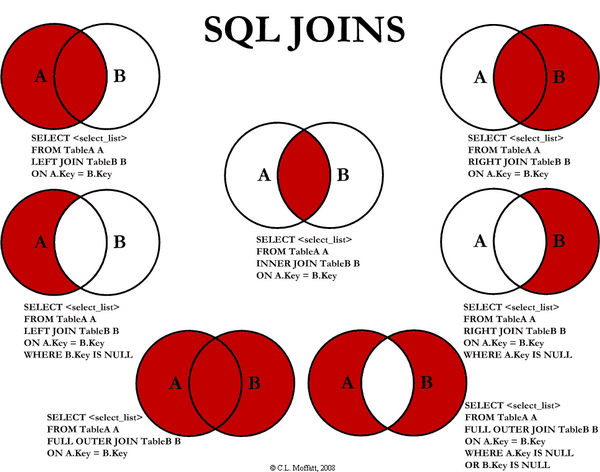
\includegraphics[scale=0.5]{./Figures/joins}
\end{figure}
}

%%%%%%%%%%%%%%%%%%%%%%%%%%%%%%%%%%%%%%%%%%%%%%%%%%%%%%%%%%
\frame {\frametitle{Grouping and Aggregation in MapReduce}
%%%%%%%%%%%%%%%%%%%%%%%%%%%%%%%%%%%%%%%%%%%%%%%%%%%%%%%%%%
  \begin{itemize}
    
  \item \textbf{Let $R(A,B,C)$ be a relation to which we apply
      $\gamma_{A,\theta(B)}(R)$}
    \begin{itemize}
    \item The map operation prepares the grouping
    \item The grouping is done by the framework
    \item The reducer computes the aggregation
    \item Simplifying assumptions: one grouping attribute and
      one aggregation function
    \end{itemize}
    
    \vspace{20pt}
    
  \item \textbf{MapReduce implementation of $\gamma_{A,\theta(B)}(R)$}\footnote{Note here that we are also projecting.}
    \begin{itemize}
    \item[\texttt{Map}:]
      \begin{itemize}
      \item For each tuple $(a,b,c)$ emit the key/value pair $(a,b)$
      \end{itemize}
    \item[\texttt{Reduce}:]
      \begin{itemize}
      \item Each key $a$ represents a group
      \item Apply $\theta$ to the list $[b_1,b_2,\cdots,b_n]$
      \item Emit the key/value pair $(a,x)$ where $x=\theta([b_1,b_2,\cdots,b_n])$
      \end{itemize}   
    \end{itemize}

  \end{itemize}    
}

%%%%%%%%%%%%%%%%%%%%%%%%%%%%%%%%%%%%%%%%%%%%%%%%%%%%%%%%%%


%%%%%%%%%%%%%%%%%%%%%%%%%%%%%%%%%%%%%%%%%%%%%%%%%%%%%%%%%%
% \section{References}

% \begin{frame}
%  \begin{colorblock}{blue}{lightblue}{ }
%   \begin{center}
%     \Huge \textbf{\texttt{References}}
%   \end{center}
%   \end{colorblock}
% \end{frame}

% \begin{frame}[allowframebreaks]{References}
% \bibliographystyle{plain} 
% \bibliography{references} 
% \end{frame}
%%%%%%%%%%%%%%%%%%%%%%%%%%%%%%%%%%%%%%%%%%%%%%%%%%%%%%%%%%

\end{document}
